\documentclass[varwidth,border=10pt]{standalone}

\usepackage[aboveskip=1pt,labelfont=bf,labelsep=period,justification=raggedright,singlelinecheck=off]{caption}
\usepackage{amsmath}
\usepackage{tikz}
\usepackage{tikz-cd}
\usetikzlibrary{matrix,arrows,positioning,calc,shapes,arrows.meta}
\usepackage{xstring}
\tikzset{  
	-Latex,auto,node distance =1.5 cm and 1.3 cm, thick,% node distance is the distance between one node to other, where 1.5cm is the length of the edge between the nodes  
	state/.style ={ellipse, draw, minimum width = 0.9 cm}, % the minimum width is the width of the ellipse, which is the size of the shape of vertex in the node graph  
	point/.style = {circle, draw, inner sep=0.18cm, fill, node contents={}},  
	bidirected/.style={Latex-Latex,dashed}, % it is the edge having two directions  
	el/.style = {inner sep=2.5pt, align=right, sloped}  
} 
%\usepackage[subrefformat=parens, labelfont=up]{subcaption}
%\usepackage{cleveref}
%\crefname{thm}{Theorem}{Theorems}
\setlength{\textwidth}{\dimexpr 6in\relax}
\usepackage{makecell}



\newcommand{\bbB}{\mathbb{B}}
\newcommand{\bL}{\mathbb{L}}
\newcommand{\bU}{\mathbb{U}}

\newcommand{\cL}{\mathcal{L}}
\newcommand{\cM}{\mathcal{M}}

\newcommand{\Targets}{\mathbf{T}}
\newcommand{\Sources}{\mathbf{S}}

\newcounter{countitems}


\newcommand{\boolf}{{\mathfrak 0}}
\newcommand{\boolt}{{\mathfrak 1}}

\newcommand{\bzero}{{\bf 0}}
\newcommand{\bone}{{\bf 1}}

\newcommand{\setof}[1]{\left\{ {#1}\right\}}
\newcommand{\setdef}[2]{\left\{{#1}\,\left|\,{#2}\right.\right\}}

\usepackage[subrefformat=parens, labelfont=up]{subcaption}

\begin{document}

\begin{figure}[ht]
    \centering
    \begin{subfigure}[c]{0.25\textwidth}
        \centering
        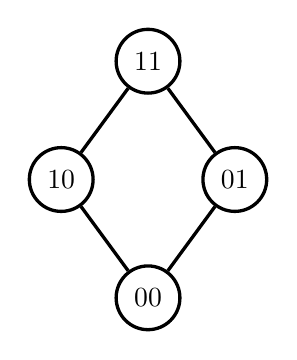
\begin{tikzpicture}[node distance = .3cm,baseline=(current bounding box.center)]
            \tikzset{my node/.style = {circle, draw, very thick, inner sep=4pt, minimum size=0pt}}
            \tikzset{my edge/.style = {-, very thick}}
            \node[my node] (1)[]{$11$};
            \node[my node] (2) [below left=0.9 and 0.5 of 1] {$10$};
            \node[my node] (3) [below right=0.9 and 0.5 of 1] {$01$};
            \node[my node] (4) [below left=0.9 and 0.5 of 3] {$00$};
            \draw[my edge] (1) -- (2);
            \draw[my edge] (1) -- (3);
            \draw[my edge] (2) -- (4);
            \draw[my edge] (3) -- (4);
        \end{tikzpicture}
        \caption{}
        \label{fig:P}
    \end{subfigure}
    \hfill
    \begin{subfigure}[c]{0.3\textwidth}
        \centering
        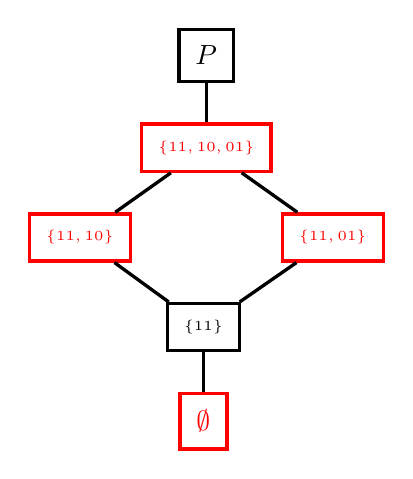
\begin{tikzpicture}[node distance = .5cm,baseline=(current bounding box.center)]
            \tikzset{my node/.style = {rectangle, draw, very thick, inner sep=6pt, minimum size=0pt}}
            \tikzset{my edge/.style = {-, very thick}}
            \node[my node] (1)[]{$P$};
            \node[my node,red] (2) [below=of 1]{\tiny $\{11,10,01\}$};
            \node[my node,red] (3) [below left=0.5 and 0.1 of 2]{\tiny $\{11,10\}$};
            \node[my node,red] (4) [below right=0.5 and 0.1 of 2]{\tiny $\{11,01\}$};
            \node[my node] (5) [below left=0.5 and 0.5 of 4]{\tiny $\{11\}$};
            \node[my node,red] (6) [below=of 5]{$\emptyset$};
            \draw[my edge] (1) -- (2);
            \draw[my edge] (2) -- (3);
            \draw[my edge] (2) -- (4);
            \draw[my edge] (3) -- (5);
            \draw[my edge] (4) -- (5);
            \draw[my edge] (5) -- (6);
        \end{tikzpicture}
        \caption{}
        \label{fig:UP}
    \end{subfigure}
    \hfill
    \begin{subfigure}[c]{0.25\textwidth}
        \centering
        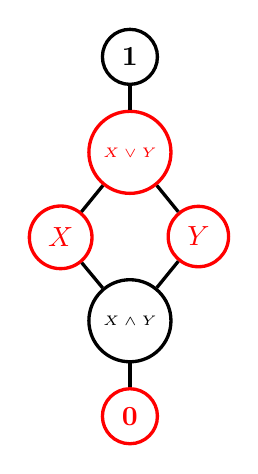
\begin{tikzpicture}[node distance = .3cm,baseline=(current bounding box.center)]
            \tikzset{my node/.style = {circle, draw, very thick, inner sep=4pt, minimum size=0pt}}
            \tikzset{my edge/.style = {-, very thick}}
            \node[my node] (1) { $\bone$ };
            \node[my node, red] (2) [below=of 1] {\tiny $X \vee Y$};
            \node[my node, red] (3) [below left=0.4 and 0.2 of 2] {$X$};
            \node[my node, red] (4) [below right=0.4 and 0.2 of 2] {$Y$};
            \node[my node] (5) [below left=0.4 and 0.2 of 4] {\tiny $X \wedge Y$};
            \node[my node, red] (6) [below=of 5] {$\bzero$};
            \draw[my edge] (1) -- (2);
            \draw[my edge] (2) -- (3);
            \draw[my edge] (2) -- (4);
            \draw[my edge] (3) -- (5);
            \draw[my edge] (4) -- (5);
            \draw[my edge] (5) -- (6);
        \end{tikzpicture}
        \caption{}
        \label{fig:L}
    \end{subfigure}
    \par\bigskip
    \begin{subfigure}[c]{0.25\textwidth}
        \centering
        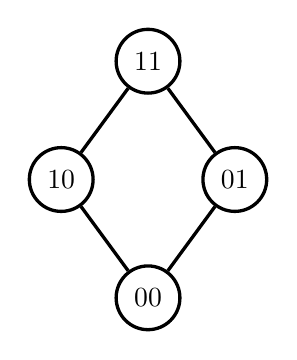
\begin{tikzpicture}[node distance = .3cm,baseline=(current bounding box.center)]
            \tikzset{my node/.style = {circle, draw, very thick, inner sep=4pt, minimum size=0pt}}
            \tikzset{my edge/.style = {-, very thick}}
            \node[my node] (1)[]{$11$};
            \node[my node] (2) [below left=0.9 and 0.5 of 1] {$10$};
            \node[my node] (3) [below right=0.9 and 0.5 of 1] {$01$};
            \node[my node] (4) [below left=0.9 and 0.5 of 3] {$00$};
            \draw[my edge] (1) -- (2);
            \draw[my edge] (1) -- (3);
            \draw[my edge] (2) -- (4);
            \draw[my edge] (3) -- (4);
        \end{tikzpicture}
        \caption{}
        \label{fig:P2}
    \end{subfigure}
    \hfill
    \begin{subfigure}[c]{0.3\textwidth}
        \centering
        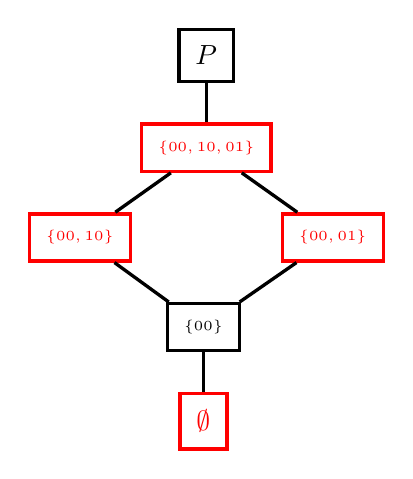
\begin{tikzpicture}[node distance = .5cm,baseline=(current bounding box.center)]
            \tikzset{my node/.style = {rectangle, draw, very thick, inner sep=6pt, minimum size=0pt}}
            \tikzset{my edge/.style = {-, very thick}}
            \node[my node] (1)[]{$P$};
            \node[my node,red] (2) [below=of 1]{\tiny $\{00,10,01\}$};
            \node[my node,red] (3) [below left=0.5 and 0.1 of 2]{\tiny $\{00,10\}$};
            \node[my node,red] (4) [below right=0.5 and 0.1 of 2]{\tiny $\{00,01\}$};
            \node[my node] (5) [below left=0.5 and 0.5 of 4]{\tiny $\{00\}$};
            \node[my node,red] (6) [below=of 5]{$\emptyset$};
            \draw[my edge] (1) -- (2);
            \draw[my edge] (2) -- (3);
            \draw[my edge] (2) -- (4);
            \draw[my edge] (3) -- (5);
            \draw[my edge] (4) -- (5);
            \draw[my edge] (5) -- (6);
        \end{tikzpicture}
        \caption{}
        \label{fig:JP}
    \end{subfigure}
    \hfill
    \begin{subfigure}[c]{0.2\textwidth}
        \centering
        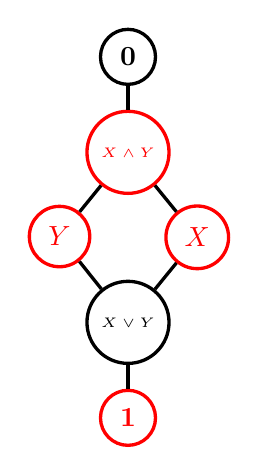
\begin{tikzpicture}[node distance = .3cm,baseline=(current bounding box.center)]
            \tikzset{my node/.style = {circle, draw, very thick, inner sep=4pt, minimum size=0pt}}
            \tikzset{my edge/.style = {-, very thick}}
            \node[my node] (1) { $\bzero$ };
            \node[my node, red] (2) [below=of 1] {\tiny $X \wedge Y$};
            \node[my node, red] (3) [below left=0.4 and 0.2 of 2] {$Y$};
            \node[my node, red] (4) [below right=0.4 and 0.2 of 2] {$X$};
            \node[my node] (5) [below left=0.4 and 0.2 of 4] {\tiny $X \vee Y$};
            \node[my node, red] (6) [below=of 5] {$\bone$};
            \draw[my edge] (1) -- (2);
            \draw[my edge] (2) -- (3);
            \draw[my edge] (2) -- (4);
            \draw[my edge] (3) -- (5);
            \draw[my edge] (4) -- (5);
            \draw[my edge] (5) -- (6);
        \end{tikzpicture}
        \caption{}
        \label{fig:U}
    \end{subfigure}
\label{fig1}
\end{figure}
\end{document}